\chapter{Health sector \& Data}

In this chapter, we provide an overview of data from the health sector and the actors involved in it, by presenting the components of a health system and the types of data generated by each activity. In the second part, we will move on to the multiple electronic records used in the healthcare.

\section{A title}
Healthcare is a multi-dimensional system established with the sole aim for the prevention, diagnosis, and treatment of health-related issues or impairments in humans. There is three components of a healthcare system\cite{dash2019big}:
\begin{itemize}
    \item The health professionals (physicians or nurses): belong to various health sectors like dentistry, medicine, midwifery, nursing, psychology, physiotherapy, and many others.
    \item Health facilities (clinics, hospitals for delivering medicines and other diagnosis or treatment technologies).
    \item Financing institution supporting the former two.
  \end{itemize}
  Healthcare is required at several levels depending on the urgency of situation:
  \begin{enumerate}
    \item \textbf{\textit{Primary care:}} Professionals serve it as the first point of consultation.
    \item \textbf{\textit{Secondary care:}} acute care requiring skilled professionals.
    \item \textbf{\textit{Tertiary care:}} advanced medical investigation and treatment.
    \item \textbf{\textit{Quaternary care:}} highly uncommon diagnostic or surgical procedures.
  \end{enumerate}
 At all these levels, the health professionals are responsible for different kind of information such as a patient's medical history (diagnosis and prescriptions related data), medical and clinical data (like data from imaging and laboratory examinations), and other private or personal medical data


Regardless of what form it takes, data has the potential to tell stories, identify cost savings and efficiencies, new connections and opportunities, and enable improved understanding of the past to shape a better future\cite{Zillner2016}.

The term “big data” has become a buzzword in recent years, with its usage frequency having doubled each year in the last few years according to common search engines (Figure \ref{fig:bigDataGoogleScholar}).

\begin{figure}[h!]
    \center
    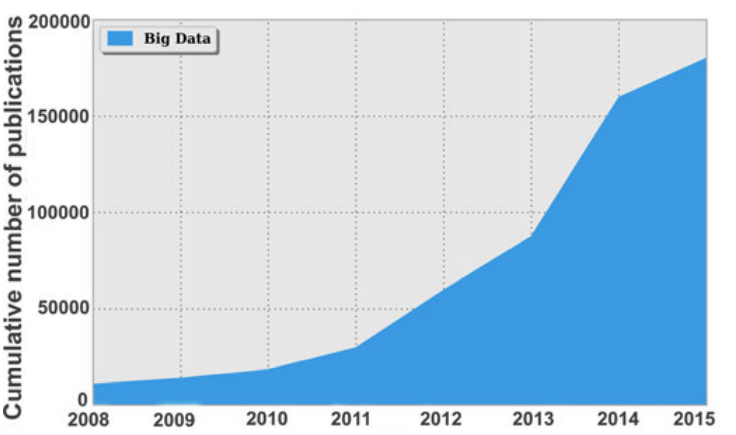
\includegraphics[width=0.75\textwidth]{images/chapter1/publication_big_data.PNG}
    \caption{Cumulative number of publications referring to “big data” indexed by Google Scholar.}
    \label{fig:bigDataGoogleScholar}
  \end{figure}
 
Big data is a vague term with a definition that is not universally agreed upon. A definition by Demchenko et al\cite{demchenko2012addressing} who define Big Data by five V’s: Volume, Velocity, Variety, Veracity, and Value. Volume pertains to vast amounts of data, Velocity applies to the high pace at which new data is generated, Variety pertains to the level of complexity of the data, Veracity measures the genuineness of data, and Value evaluates how good the quality of the data is in reference to the intended results.


If we trace the relationship between the use of the term big data per health research , we can easily infer the growth of medical informatics (Figure \ref{fig:bigDataHealthResearch}). Big data in health is concerned with meaningful datasets that are too big, too fast, and too complex for healthcare providers to process and interpret with existing tools\cite{andreu2015big}.
\begin{figure}[h!]
    \center
    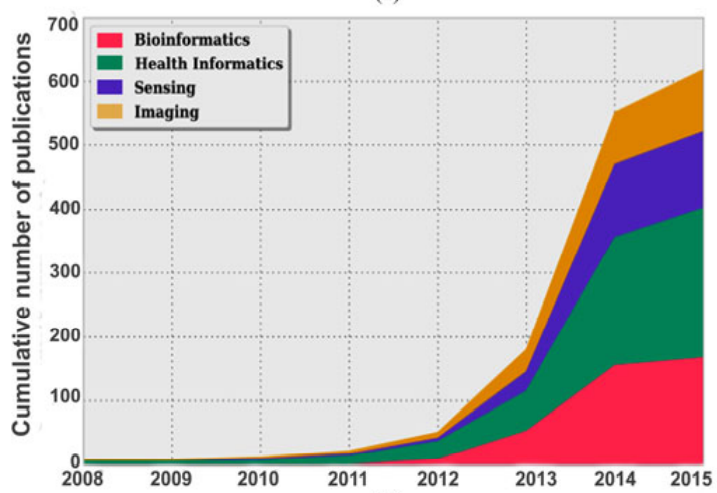
\includegraphics[width=0.75\textwidth]{images/chapter1/health_publication_bigData.PNG}
    \caption{Cumulative number of publications per health research
    area referring to “big data,” as indexed in IEEE Xplore, ACM Digital library, PubMed (National Library of Medicine, Bethesda, MD), Web of Science, and Scopus.}
    \label{fig:bigDataHealthResearch}
  \end{figure}

  \newpage
There are numerous current areas of research within the field of Health Informatics, including Bioinformatics, Image Informatics (e.g. Neuroinformatic), Clinical Informatics, Public Health Informatics, and also Translational BioInformatics (TBI). Research done in Health Informatics (as in all its subfields) can range from data acquisition, retrieval, storage, analytics employing data mining techniques, and so on.
\bigbreak
Data gathered for Health Informatics research does exhibit many of these qualities. Big Volume comes from large amounts of records stored for patients: for example, in some datasets each instance is quite large (e.g. datasets using MRI images or gene microarrays for each patient), while others have a large pool with which to gather data (such as social media data gathered from a population). Big Velocity occurs when new data is coming in at high speeds, which can be seen when trying to monitor real-time events whether that be monitoring a patient’s current condition through medical sensors or attempting to track an epidemic through multitudes of incoming web posts (such as from Twitter). Big Variety pertains to datasets with a large amount of varying types of independent attributes, datasets that are gathered from many sources (e.g. search query data comes from many different age groups that use a search engine), or any dataset that is complex and thus needs to be seen at many levels of data throughout Health Informatics.

\newpage
Schematically, several health-related activities can be distinguished\cite{martigneneVisualisationUnifieeDonnees}:
\begin{itemize}
  \item Pre-admission, admission and administrative discharge activities.
  \item T2A invoicing or valuation activities.
  \item Care activities in the accommodation service.
  \item Activities in operating theaters and technical platforms.
  \item Laboratory activities.
  \item Imaging activities.
\end{itemize}

For each activity, different types of data are generated. In France and most developed countries, the following data is collected and digitally available (in chronological order)\cite{ATIHAgenceTechnique,boracle2009detection}:
\label{chap:healthData}
\begin{enumerate}
  \item \textbf{Administrative data} related to patient movements (identity, dates, places, etc.), demographic (age, sex, place of residence, etc.) and insurance (health coverage, etc.).
  \item \textbf{Results of biological analyses}, generally taken by nurses and analyzed by professionals or by robots.
  \item \textbf{Medical data} produced automatically by autonomous medical devices. These devices can be implantable or external.
  \item \textbf{Data relating to the drugs administered to the patient},
  generally by nurses or doctors, possibly as part of a diagnostic or therapeutic procedure.
  \item \textbf{Data relating to medical devices} implanted in the patient during surgery.
  \item \textbf{Data relating to medical procedures}, whether diagnostic or therapeutic. These data are generally coded by the producer, sometimes by the machine which produces them.
  \item \textbf{Comments} in free text, possibly formalized in letters or reports.
  \item \textbf{Medical diagnoses}, coded a posteriori by the doctors who treated the patient, or by specialized technicians reading the letters\cite{emmanuelchazardReutilisationFouilleDonnees2017}.
\end{enumerate}


\newpage

This data can be structured (which can be used directly by an algorithm) or unstructured (they are stored without a predefined format, such as the text of reports or medical letters, and are interpreted by humans). Machines generally produce raw structured information (eg medical biology measurements), while healthcare professionals exchange unstructured information with high interpretative value (eg a diagnosis). 
Medical records are created by aggregating information from different sources: (Table \ref{tab:sourceTable}) gives an overview of this data\cite{martigneneVisualisationUnifieeDonnees}. 


\begin{table}[h!]
    \centering
    \begin{tabular}{|m{0.45\linewidth}|m{0.20\linewidth}|m{0.35\linewidth}|}
        \hline
        Category                                         & Nature                                                        & Structure                                                   \\
        \hline
        \textbf{Administrative data}                                           & Values, Text                                 & Structured                                       \\
        \hline
        \textbf{Communications between caregivers} (Transmissions and medical observations, medical letters, reports)                      & Text              & Unstructured                                               \\
        \hline
        \textbf{Data managed by centralized pharmacies}                       & Values         & Structured                    \\
        \hline
        \textbf{Medical biology results}                               & Values, Text & Structured                           \\
        \hline
        \textbf{Data from monitoring devices}     & Values                                                         & Structured                                                      \\
        \hline
        \textbf{Image Data Images}                             & Images, Text                                                & Unstructured                               \\
        \hline
        \textbf{PMSI data and codes}  & Codes, Values                                                        & Structured                                              \\
                               
        \hline
    \end{tabular} 

    \caption{Origin, nature and structure of medical record data.}
    \label{tab:sourceTable}
\end{table}


\section{Medical records management}
Self-tracking and documenting information about aspects of one’s personal and daily life has a long history. It is an effective method which helps us to learn more about ourselves, rather than depending on our limited memory\cite{alrehielyEvaluatingDifferentVisualization}.


The medical record is a multifunctional document that is used to communicate and document critical information about patients’ medical care among health care professionals. Comprehensive medical records are a cornerstone in the quality and efficiency of patient care during the hospitalization and in subsequent follow-up visits, as they can provide a complete and accurate chronology of treatments, patient results and future plans for care\cite{wong2009developing}, it involves many kinds of records, including patient charts, x-rays, images, scans, and even emails. Additionally, it involves making sure all of these items are accessible, safe, and secure.
There are multiple electronic records used in the healthcare.
\subsection{Electronic medical record}
Electronic medical record (EMR) systems, defined as "an electronic record of health-related information on an individual that can be created, gathered, managed, and consulted by authorized clinicians and staff within one health care organization,"  have the potential to provide substantial benefits to physicians, clinic practices, and health care organizations. 

It  is a digital version of the paper medical record that has been used for years and it will contain the patient’s medical and surgical history, allergy information, treatment history, current, and past prescriptions, and other pertinent information that can be used in making future medical decisions\cite{WheelWhatAre}. These systems can facilitate workflow and improve the quality of patient care and patient safety\cite{ElectronicMedicalRecord}.

\subsection{Electronic health record}
An Electronic Health Record (EHR) is an electronic version of a patient's medical history, that is maintained by the provider over time, and may include all of the key administrative clinical data relevant to that persons care under a particular provider, including demographics, progress notes, problems, medications, vital signs, past medical history, immunizations, laboratory data and radiology reports. The EHR automates access to information and has the potential to streamline the clinician's workflow.  It also has the ability to support other care-related activities directly or indirectly through various interfaces, including evidence-based decision support, quality management, and outcomes reporting. 
 
EHRs are the next step in the continued progress of healthcare that can strengthen the relationship between patients and clinicians.  The data, and the timeliness and availability of it, will enable providers to make better decisions and provide better care\cite{ElectronicHealthRecords}.


\subsection{The Difference Between EMR \& EHR}
Both the EMR and EHR contain electronic versions of a patient's medical history. Most of the information in an EMR goes into an EHR.


The EMR can contain medical history, diagnoses, medications, immunizations and dates, allergies, etc. Often, a patient needs to ask for a printed copy of an EMR to share with another medical provider.


The EHR contains similar details as the EMR, but also other relevant data like information from wearable devices, demographics, and insurance information. It can also contain lab data and imaging reports that come from other offices or practices. Assuming the software is compatible, other offices and practices can access the information within an EHR to help coordinate care and make clinical decisions\cite{KeyMaintainingMedical} (Table \ref{tab:EMRvsEHR}) gives an overview of this difference:
\begin{table}[h!]
    \centering
    \begin{tabular}{|m{0.50\linewidth}|m{0.50\linewidth}|}
        \hline
        \textbf{EMR (electronic medical record)}                             & \textbf{EHR (electronic health record)}                                  \\
        
        \hline
        Medical and clinical data gathered in one provider's office         & Medical and clinical data gathered from many providers' offices and hospitals     \\
        
        \hline
        Narrower view                       & Broader view        \\
        
        \hline
        Digital version of a paper chart in one office                       & Digital version of varied health information        \\
        
        \hline
        Not designed for sharing                             & Designed for sharing outside of an individual medical practice       \\
        
        \hline
        Providers use mainly for diagnosis and treatment     & Providers have access to many diagnostic tools to make decisions       \\
        
        \hline
    \end{tabular} 

    \caption{EMR vs. EHR: Similarities and Differences.}
    \label{tab:EMRvsEHR}
\end{table}


\subsection{Personal health record}
Electronic Personal Health Records (ePHRs) are a representation of health records connected to the care of a patient and are managed by the patient\cite{demirisPatientcenteredApplicationsUse2008}, unlike EHRs, which are managed by health care providers. ePHRs allow healthcare consumers the luxury of deciding which health information to share with healthcare providers\cite{tangPersonalHealthRecords2006}. Ozok et al.\cite{PaperbasedComputerbasedRecords} defined ePHR systems as patient centric, multi-functional, health management systems developed for managing and storing lifelong personal health information for various purposes from chronic to critical, medical and preventive care\cite{alsahafiOverviewElectronicPersonal2018}.

The information in an EHR is keyed in by healthcare providers and is only accessible to healthcare providers. In addition, an EHR might only contain information from a single healthcare provider. On the other hand, an individual will retain control of their own ePHR, which might encompass health information from different sources, such as various healthcare providers, as well as from the patient, as integrated ePHRs have the capability to incorporate data from different sources. Thus, at any one time, there may be various EHRs for one person but only one ePHR\cite{alsahafiOverviewElectronicPersonal2018}.
\begin{figure}[h!]
  \center
  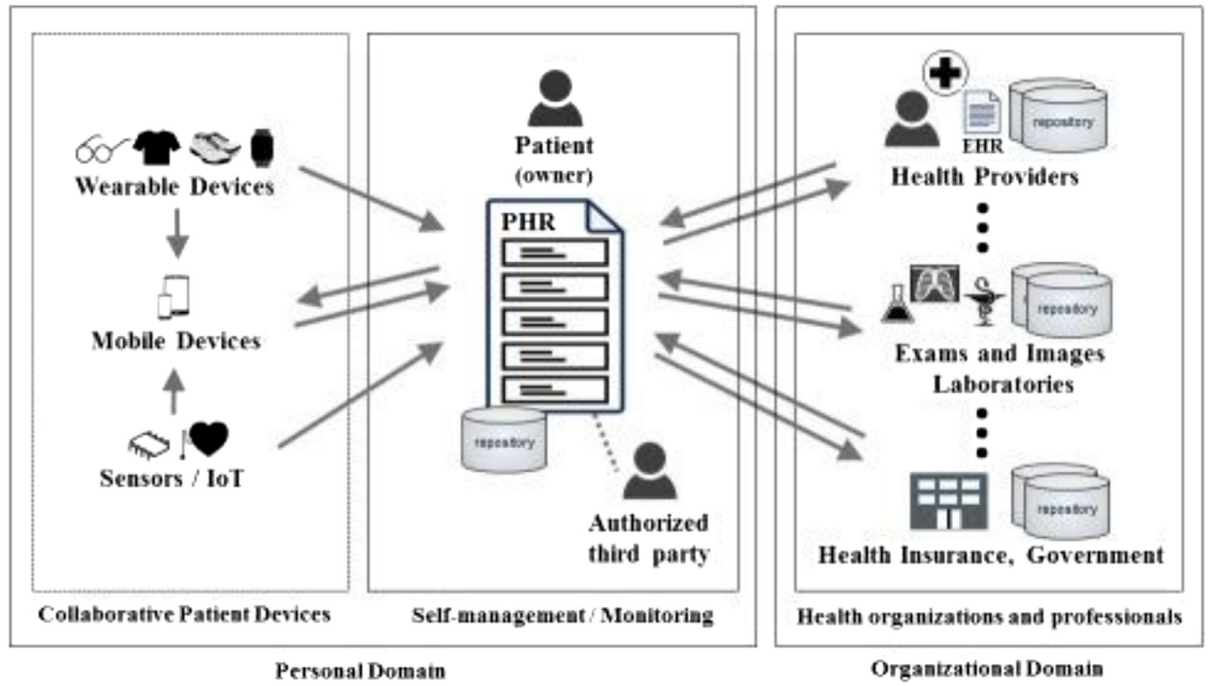
\includegraphics[width=0.75\textwidth]{images/chapter1/phr_ehr.PNG}
  \caption{Difference between an EHR and ePHR (Taken from \cite{alsahafiOverviewElectronicPersonal2018}).}
  \label{fig:ehrvsphr}
\end{figure}

\section{Security in medical records management}
The actual technology of an electronic medical record seems to be falling into place. As the world moves more toward the use of telemedicine to preclude the movement of patients to more advanced facilities, the need for a fully functioning medical record is paramount.
One of the important ethical issues in electronic records management involves privacy. Privacy is the “claim of individuals to be left alone, free from surveillance or interference from other individuals, organizations, including state” (Laudon and Laudon 2005:159), privacy deals with the collection and use or misuse of data. Data is constantly being collected and stored on each of us. This data is often distributed over easily accessed networks and without our knowledge or consent\cite{ngoepeSecurityPrivacyEthics2011}.
 
 
There are a number of security dilemmas in electronic records management. There can be illegal access and use of records, data alteration and destruction (Stair and Reynolds 2006: 583).

\bigbreak
Typical cross-organisational e-health applications are\cite{ruotsalainenCrossplatformModelSecure2004}: 
\begin{itemize}
\item sharing of patient records among different healthcare professionals; 
\item access to distributed EHRs any place and any time; 
\item on-line teleconsultation, telemonitoring and assistance; 
\item patient—doctor consultation services;
\item patients’ access to their own EHRs.
\end{itemize}

\bigbreak
That is why Electronic health records management attracts significant international interest and sets the scenery for the establishment of a distributed, coalition-based, security policy enhanced records exchange framework among different medical domains. Several European projects have proposed candidate solutions for secure inter-operations between medical domains. In the HARP project, security profiles related to access rights are dynamically downloaded to the client side. The MEDITRAV EUproject attempts to overcome national or linguistic barriers by adopting the solution of a multilingual portable personal record. These approaches, pose mainly their research effort on the security requirements for effective electronic health record management, still they confront mainly to stable infrastructures\cite{belsisPervasiveSecureElectronic2005}.